
\chapter{Week 3 \\ Hyperparameter Tuning}


% - Hyperparameter Tuning -------------------------------------------------------
\section{Hyperparameter Tuning}

Parameters to tune:
\begin{tabular}{|l|l|}
    \hline
    Parameter & Priority \\
    \hline
    $\alpha$ & 1 \\
    \hline
    $\beta$ & 2 \\
    \hline
    $\beta_1, \beta_2, \epsilon$ & 4 \\
    \hline
    numLayers & 3 \\
    \hline
    numHiddenUnits & 2 \\
    \hline
    learningRateDecay & 3 \\
    \hline
    miniBatchSize & 2 \\
    \hline
\end{tabular}

\subsection*{Tuning Parameters}

\subsubsection*{Random Sampling}

Selecting values to try from a grid used to be common practice:
\begin{tikzpicture}
    % Draw square
    \draw (0,0) rectangle (7,7);
    
    % Add labels
    \node[rotate=90, anchor=center] at (-0.5,3.5) {Hyperparameter 1};
    \node[anchor=center] at (3.5,7.5) {Hyperparameter 2};
    
    % Draw the 5x5 grid inside the square
    \foreach \x in {1.4, 2.8, 4.2, 5.6} {
        \foreach \y in {1.4, 2.8, 4.2, 5.6} {
            \fill (\x,\y) circle (2pt);
        }
    }
\end{tikzpicture}

A better approach is to sample randomly:


\begin{tikzpicture}
    % Draw square
    \draw (0,0) rectangle (7,7);
    
    % Add labels
    \node[rotate=90, anchor=center] at (-0.5,3.5) {Hyperparameter 1};
    \node[anchor=center] at (3.5,7.5) {Hyperparameter 2};
    
    % Define the coordinates in an array
    \def\pointslist{
        (1,2), (5,5.5), (2.5,6.2), (6,1.5), (3.7,2.3), 
        (1.5,5), (2,1), (6.5,6), (5.5,1.5), (3,5.5),
        (4.5,3), (1.2,3.5), (6.2,4), (5.8,2.7), (2.2,4.6), 
        (4,6), (3.5,1.2), (6.5,3), (5,3.5), (1.8,6),
        (4,2.5), (2.5,2), (3.5,4.5), (4.8,5), (2.8,1.5)
    }
    
    % Loop through each coordinate and plot the point
    \foreach \point in \pointslist {
        \fill \point circle (2pt);
    }
\end{tikzpicture}

If only one of the parameters turns out to be unimportant, then at least with the random sampling we end up 
trying many more values for the important parameter.

\subsubsection*{Coarse to fine}

If after a coarse search in the space of all hyperparameters you find that the best combinations of values
lie in a smaller part of that space, zoom in to that subspace and and do a more fine grained search.


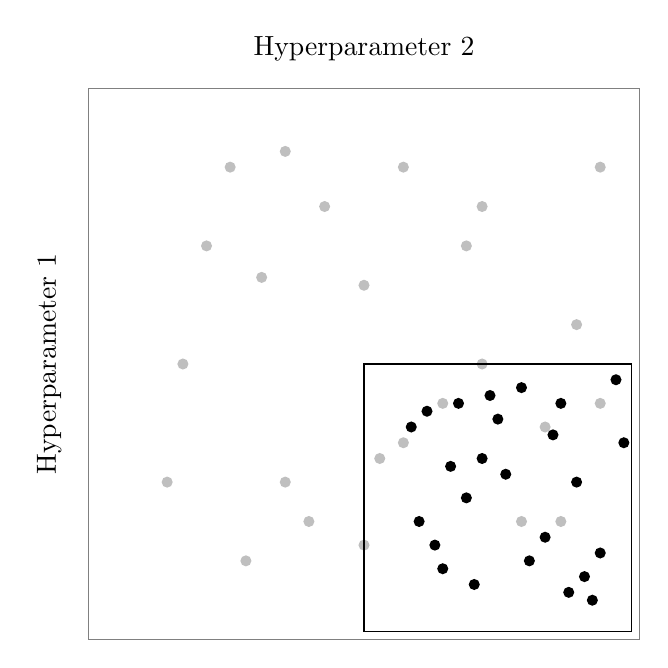
\begin{tikzpicture}
    % Draw square
    \draw[draw=gray] (0,0) rectangle (7,7);
    
    % Add labels
    \node[rotate=90, anchor=center] at (-0.5,3.5) {Hyperparameter 1};
    \node[anchor=center] at (3.5,7.5) {Hyperparameter 2};
    
    % Define the coordinates in an array
    \def\pointslist{
        (1,2), (5,5.5), (2.5,6.2), (6,1.5), (3.7,2.3), 
        (1.5,5), (2,1), (6.5,6), (5.5,1.5), (3,5.5),
        (4.5,3), (1.2,3.5), (6.2,4), (5.8,2.7), (2.2,4.6), 
        (4,6), (3.5,1.2), (6.5,3), (5,3.5), (1.8,6),
        (4,2.5), (2.5,2), (3.5,4.5), (4.8,5), (2.8,1.5)
    }
    
    % Loop through each coordinate and plot the point
    \foreach \point in \pointslist {
        \fill[fill=lightgray] \point circle (2pt);
    }

    \def\pointslistx{
    (4.2,1.5), (6.3,0.8), (5,2.3), (6.5,1.1), (4.7,3),
    (6.8,2.5), (4.9,0.7), (5.5,3.2), (4.3,2.9), (5.6,1),
    (5.3,2.1), (6.1,0.6), (6.7,3.3), (4.5,0.9), (6.2,2),
    (5.8,1.3), (6,3), (4.6,2.2), (4.1,2.7), (4.8,1.8),
    (5.2,2.8), (6.4,0.5), (5.1,3.1), (5.9,2.6), (4.4,1.2)
    }
 
    % Loop through each coordinate and plot the point
    \foreach \point in \pointslistx {
        \fill[fill=black] \point circle (2pt);
    }

    \draw[draw=black] (3.5,3.5) rectangle (6.9, 0.1);

\end{tikzpicture}

\section{Using an Appropriate Scale to pick Hyperparameters}

There are several ways to pick hyperparameters at random, depending on their scale.

\subsection*{Sampling uniformly at random }

Examples:

Number of hiddenunits in layer $l$: $n^{[l]} \in [50,100]$

Number of layers in a network, $L: L \in [2,4]$

\subsection*{Sampling from a logarithmic distribution}

Example:

Sample learning rate between $0.0001$ and $1$

\[ \{r | r \in \mathbb{R}, -4 \leq r \leq 0\} \]
\[ \alpha = 10^r \]

Generally, sampling a value $v$ between $10^a$  and $10^b$:

\[ \{ r | r \in \mathbb{R}, a \le r \le b\} \]
\[ v = 10^r \]

\subsection*{Sampling hyperparameters for exponentially weighted averages}

Sample $\beta$ between $0.9$ and $0.999$

Sample $(1 - \beta)$  from $0.1$ to $0.001$ (see log sampling above)


\section{Hyperparameters Tuning in Practice}

Intuitions can transfer between domains.
Intutions can go stale. Re-evaluate hyperparameters occasionally.

\subsection*{Babysitting one model}

\includegraphics[width=0.3\linewidth]{images/single_model.png}

When training over a long time, adjust parameters as training progresses.

\subsection*{Training many models in parallel}

\includegraphics[width=0.3\linewidth]{images/parallel_models.png}

Allows you to test many parameter values at the same time, pick the best in the end.




% - Batch Normalization ---------------------------------------------------------

\section{Batch Normalization - Normalizing Activations in a Network}

\subsection*{Logistic regression}

For a single neuron we have seen how we can normalize the inputs

\begin{tikzpicture}[
    >={Latex[scale=2]},
    % Define the style for the nodes
    xory/.style={circle, minimum size=0.8cm, inner sep=0pt},
    neuron/.style={circle, draw=black, minimum size=0.8cm, inner sep=0pt},
    layer/.style={anchor=center, nodes=neuron, node distance=0.8cm}
]

    \node[xory] (x1) {$x_1$};
    \node[xory, below=0.7cm of x1] (x2) {$x_2$};
    \node[xory, below=0.7cm of x2] (x3) {$x_3$};
    \node[neuron, right=2cm of x2] (n1) {};
    \node[xory, right=0.5cm of x1] (formula) {$w,b$};
    \node[xory, right=1.5cm of n1] (y1) {$\hat{y}$};

    \draw[->] (x1) -- (n1);
    \draw[->] (x2) -- (n1);
    \draw[->] (x3) -- (n1);
    \draw[->] (n1) -- (y1);

\end{tikzpicture}

We calculate mean and variance:

\[ \mu = \frac{1}{m} \sum_{i=1}^m x^{(i)} \]
\[ \sigma^2 = \frac{1}{m} \sum_{i=1}^m (x^{(i)} - \mu)^2 \]

Then normalize $X$:

\[ \hat{X} = \frac{X - \mu}{\sqrt{\sigma^2 + \epsilon}} \]

\subsection*{Deeper Networks}

\begin{tikzpicture}[
    >={Latex[scale=2]},
    % Define the style for the nodes
    xory/.style={circle, minimum size=0.8cm, inner sep=0pt},
    neuron/.style={circle, draw=black, minimum size=0.8cm, inner sep=0pt},
    layer/.style={anchor=center, nodes=neuron, node distance=0.8cm}
]

    % input layer
    \node[xory] (x1-1) {$x_1$};
    \node[xory, below=0.7cm of x1-1] (x1-2) {$x_2$};
    \node[xory, below=0.7cm of x1-2] (x1-3) {$x_3$};

    % hidden layers
    \foreach \i [remember=\i as \lasti (initially 1)] in {2, 3, 4} {
        \node[neuron, right=1.5cm of x\lasti-1] (x\i-1) {};
         \node[neuron, right=1.5cm of x\lasti-2] (x\i-2) {};
         \node[neuron, right=1.5cm of x\lasti-3] (x\i-3) {};

         \foreach \j in {1,...,3} {
             \foreach \k in {1,...,3} {
                 \draw[->] (x\lasti-\k) -- (x\i-\j);
             }
         }
    }

    %output
    \node[neuron, right=1.5cm of x4-2] (y1) {};
    \draw[->] (x4-1) -- (y1);
    \draw[->] (x4-2) -- (y1);
    \draw[->] (x4-3) -- (y1);
    \node[xory, right=0.7cm of y1] (yhat) {$\hat{y}$};
    \draw[->] (y1) -- (yhat);

\end{tikzpicture}

For any hidden layer, can we normalize $a^{[l-1]}$  so as to train $w^{[l]}, b^{[l]}$ faster?

Given some intermediate values for a layer in a neural network $\{z^{(1)}, \ldots, z^{(m)}\}$, we can normalize them:
\begin{align*}
    \mu            &= \frac{1}{m} \sum_i z^{(i)} \\
    \sigma^2       &= \frac{1}{m} \sum_i(z^{(i)} - \mu)^2 \\
    z_{norm}^{(i)} &= \frac{z^{(i)} - \mu}{\sigma} \approx \frac{z^{(i)} - \mu}{\sqrt{\sigma^2+\epsilon}} 
\end{align*}

Now we don't always want the input to the activation functions to have mean $0$ and variance $1$, so we take
\[ \tilde{z}^{(i)}=\gamma z_{norm}^{(i)} + \beta \]

where $\beta, \gamma$ are learnable parameters of the model.

Now if
\[
\begin{cases}
    \gamma &= \sqrt{\sigma^2 + \epsilon} \\
    \beta  &= \mu
\end{cases}
\]

then
\[ \tilde{z}^{(i)} = z^{(i)} \]

so any mean and variance can be learned. Batch Norm also makes the constant $b$ in the expression 
$a=Wx+b$ redundant, since it will be removed in the normalization step. The $\beta$ term will play the same role as $b$ here.

When working with mini-batches, normalization is done over each mini-batch using only the data from that mini-batch.

\subsection*{Why does Batch Norm work?}

\includegraphics[width=\linewidth]{images/learning_on_shifting_distribution.png}

A function trained on the data set on the left will not be good at predicting labels in the data set on the right. 
They come from a shifted distribution, known as a covariate shift.

Covariate shift $\implies$ a need to retrain the network.

A layer deeper than the first of a DNN suffers from covariate shift due to the shifting inputs from the previous layers:

\includegraphics[width=\linewidth]{images/nn_covariate_shift.png}

Batch norm will address this by limiting the changes in the input to a layer since variance and mean will now remain the same.

\subsection*{Batch Norm As Regularization}

\begin{itemize}
    \item Each mini-batch is scaled by the mean/variance computed on just that mini-batch.
    \item This adds some noise to the values $z^{[l]}$ within that mini-batch. So similar to dropout, it adds some noise to each hidden layer's activations.
    \item This has a slight regularization effect.
\end{itemize}

\subsection*{Batch Norm at Test Time}

At test time, $\mu$ and $\sigma$ are estimated using exponential weighted averages across mini-batches, 
so during training you keep a running average of these variables.




% - Softmax Regression ----------------------------------------------------------
\section{Softmax Regression}

Generalization of logistic regression.

The output of the final layer $L$ with $C$ outputs is computed as usual
\begin{align*}
    z^{[L]} & = W^{[L]} a^{[L-1]} + b^{[L]}   & \text{matrix of dim}(4,1)
\end{align*}

Activation function for layer $L$:
\[ t = e^{(z^{[L]})} \]
\[ a^{[L]} = \frac{e^{z^{[L]}}}{\sum_{j=1}^C t_j},\ \ a_i = \frac{t_i}{ \sum_{j=1}^C t_j} \]

So if e.g.
\[
    z^{[L]} = 
    \begin{bmatrix}
        5 \\
        2 \\
        -1 \\
        3
    \end{bmatrix}
    \implies
    t =
    \begin{bmatrix}
        e^5 \\
        e^2 \\
        e^{-1} \\
        e^3
    \end{bmatrix}
    =
    \begin{bmatrix}
        148.4 \\
        7.4 \\
        0.4 \\
        20.1
    \end{bmatrix}
\]
\[ \sum_{i=1}^4 t_i = 176.3 \]
 \[
    a^{[L]} = 
    \begin{bmatrix}
        e^5/176.3 \\
        e^2/176.3 \\
        e^{-1}/176.3 \\
        e^3/176.3
    \end{bmatrix}
    =
    \begin{bmatrix}
        0.842 \\
        0.042 \\
        0.002 \\
        0.114
    \end{bmatrix}
    , \text{  hardmax would be}
    \begin{bmatrix}
        1 \\
        0 \\
        0 \\
        0
    \end{bmatrix}
\]

Softmax generalizes logistic regression to $C$ classes. If $C=2$, softmax reduces to logistic regression.

\subsection*{Loss Function}

The loss function used for softmax is
\[ \mathcal{L}(\hat{y}, y)= -\sum_{j=1}^Cy_j \cdot log(\hat{y}_j) \]

Example:
\[
    y = 
    \begin{bmatrix}
        0 \\
        1 \\
        0 \\
        0
    \end{bmatrix}
    ,
    a^{[L]} =
    \hat{y} =
    \begin{bmatrix}
        0.3 \\
        0.2 \\
        0.1 \\
        0.4 
    \end{bmatrix}    
\]

In this case the loss function will be
\[ \mathcal{L}(\hat{y}, y) = - y_2 \cdot log(\hat{y}_2) \]

The way to minimize this is to make $\hat{y}^2$ big, which is what we want. In this case we get
\[ \mathcal{L}(\hat{y}, y) = - log(0.2) = 1.61 \]

The cost function then becomes
\[
    \mathcal{J}(W,b) = \frac{1}{m} \sum_{i=1}^m \mathcal{L}(\hat{y}^{(i)}, y^{[i)}) \]

For the whole training set with $m$ examples, $Y$ is a matrix with dimensions $(4, m)$.

\subsection*{Gradient Descent}


\[
    dz^{[L]} = \partial{\mathcal{J}}{z^{[L]}} = \hat{y} - y 
\]

\section*{Deep Learning Frameworks}

\begin{itemize}
    \item Caffe/Caffe2
    \item CNTK
    \item DL4J
    \item Keras
    \item Lasagne
    \item mxnet
    \item PaddlePaddle
    \item TensorFlow
    \item Theano
    \item Torch
\end{itemize}

\subsection*{Choosing deep learning frameworks}

\begin{itemize}
    \item Ease of programming (development + deployment)
    \item Running speed
    \item Truly open (open source with good governance)
    \item Community support
    \item Hardware support (GPUs, CPUs, TPUs)
    \item Production support (ability to easily train huge models over multiple machines)
    \item Learning curve (easy to learn)
    \item Debugging and visualization tools
    \item Popularity
\end{itemize}
